

\tikzset{every picture/.style={line width=0.75pt}} 
%set default line width to 0.75pt        

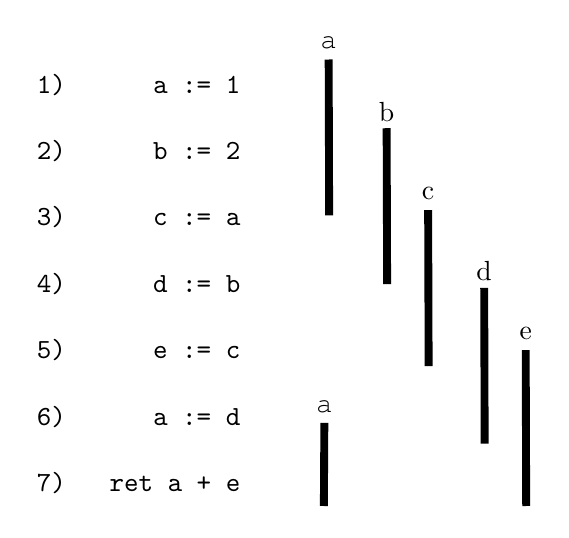
\begin{tikzpicture}[x=0.75pt,y=0.75pt,yscale=-1,xscale=1]
%uncomment if require: 
%\path (0,300); %set diagram left start at 0, and has height of 300

\draw [line width=1mm]  (168.57,24.88) -- (168.81,100.02) ;
\draw [line width=1mm]  (196.5,58) -- (196.74,133.14) ;
\draw [line width=1mm]  (166.5,200) -- (166.26,240) ;
\draw [line width=1mm]  (216.5,97.5) -- (216.74,172.64) ;
\draw [line width=1mm]  (243.5,134.86) -- (243.74,210) ;
\draw [line width=1mm]  (263.5,164.86) -- (263.74,240) ;

% Text Node
\draw (77,133) node  [align=left] {{\tt 1) \ \ \ \ \ a := 1}\\\\{\tt 2) \ \ \ \ \ b := 2}\\\\{\tt 3) \ \ \ \ \ c := a}\\\\{\tt 4) \ \ \ \ \ d := b}\\\\{\tt 5) \ \ \ \ \ e := c}\\\\{\tt 6) \ \ \ \ \ a := d}\\\\{\tt 7) \ \ ret a + e}};
% Text Node
\draw (168.57,24.88) node  [align=left] {{\fontfamily{pcr}\selectfont a}\\};
% Text Node
\draw (196.5,58) node  [align=left] {b\\};
% Text Node
\draw (166.5,200) node  [align=left] {{\fontfamily{pcr}\selectfont a}\\};
% Text Node
\draw (216.5,97.5) node  [align=left] {c\\};
% Text Node
\draw (243.5,134.86) node  [align=left] {d\\};
% Text Node
\draw (263.5,164.86) node  [align=left] {e\\};
\end{tikzpicture}
